\documentclass[11pt]{article}
\usepackage[margin=1in]{geometry}
\usepackage{amsmath,amssymb}
\usepackage{booktabs}
\usepackage{graphicx}
\usepackage{longtable}
\usepackage{siunitx}
\usepackage[table]{xcolor}
\usepackage{caption}
\usepackage[colorlinks=true,linkcolor=blue,urlcolor=blue]{hyperref}

\sisetup{detect-weight=true}
\newcommand{\halfp}{$\tfrac{1}{2}\langle111\rangle$}
\newcommand{\hkl}{$\langle100\rangle$}
\newcommand{\dnr}{\textit{d.n.r.}}
\newcommand{\nreal}{\textit{n/r}}

\title{Verification and Approximation Study for\\
       \emph{Generalized Cluster Dynamics} --- Campaign Results}
\author{RadCluster\_2\_1}
\date{10 September 2026}

\begin{document}
\maketitle

\begin{abstract}
This report collects the results of the verification campaign run in answer to
the reviewer's \S6.2 / Figure~8 critique. It reports the six experimentally
observable parameters for every campaign configuration, against the EUROFER97
measurements where a comparison is meaningful and against the fully discrete
solution for the closure verification. Section~\ref{sec:campM} adds a second campaign that separates system size from
binning, two axes the earlier tables varied together. Three defects found
\emph{by} the campaigns --- a physics channel missing from one solver path, a
dose ladder that scored the wrong dose, and a corrupted moment reaching the SIA
inventory --- are documented alongside the numbers they invalidated, because
they bear directly on what the tables may be used to claim.
\end{abstract}

\tableofcontents

%======================================================================
\section{Campaign Parameters}
%======================================================================

All runs share the EUROFER97 host declaration, fission cascade spectrum,
$G = \SI{1e-7}{dpa\per\second}$, \SI{330}{\celsius},
\texttt{full\_system} solver mode, GMRES with the Woodbury preconditioner,
\texttt{atol} $=10^{-20}$, and $i_{\rm mobile} = v_{\rm mobile} = 5$.
Table~\ref{tab:config} lists what differs.

\begin{table}[htbp]
\centering
\caption{Campaign configuration. $N_{\rm eq}$ is the main block; the
\hkl{} loop block is carried separately and adds a further $I$ equations in
discrete mode (so run D integrates 12\,006, not 8\,006).}
\label{tab:config}
\small
\begin{tabular}{llrrrrrl}
\toprule
Block & Equations & $I$ & $V$ & $i_{\rm discrete}$ & $I_{\rm bin}$ & Dose (dpa) & Scored at \\
\midrule
Table 1 (B1--B4) & bin\_moment & 80\,000 & 20\,000 & 6400--100 & 7--18 & 40 & 15.72 dpa \\
Table 2          & bin\_moment & 80\,000 & 20\,000 & 100       & 10--40 & 40 & 15.72 dpa \\
Table 3          & bin\_moment & 80\,000 & 20\,000 & 100       & 18    & 40 & 15.72 dpa \\
Table 4 (D)      & \textbf{discrete} & 4\,000 & 4\,000 & --- & --- & 2 & 2.000 dpa \\
Table 4 (C0--C4) & bin\_moment & 4\,000 & 4\,000 & 1600--5 & 2--19 & 2 & 2.000 dpa \\
\bottomrule
\end{tabular}
\end{table}

The EUROFER97 neutron measurements at \SIrange{300}{350}{\celsius}
(Table~\ref{tab:exp}) are the experimental column throughout. Their dose
coverage matters: the loop data begin at \SI{14.6}{dpa}, which is why
Tables~1--3 are scored at \SI{15.72}{dpa} and why Table~4, which runs to
\SI{2}{dpa}, cannot be compared with them at all.

\begin{table}[htbp]
\centering
\caption{EUROFER97, neutron, \SIrange{300}{350}{\celsius}. Measured ranges over
all sources in \texttt{docs/Database}.}
\label{tab:exp}
\small
\begin{tabular}{lrrr}
\toprule
Population & $n$ & Density (\SI{e21}{\per\meter\cubed}) & Diameter (nm) \\
\midrule
\halfp{} loops & 13 & 0.30 -- 34.0 & 3.3 -- 35.0 \\
\hkl{} loops   & 10 & 2.24 -- 12.0 & 2.8 -- 48.0 \\
Cavities       & 6--8 & 0.32 -- 6.30 & 1.6 -- 16.0 \\
\midrule
\multicolumn{4}{l}{Dose coverage: loops \SIrange{14.6}{32}{dpa}, cavities
\SIrange{2.7}{32}{dpa}} \\
\bottomrule
\end{tabular}
\end{table}

%----------------------------------------------------------------------
\subsection{Table 1 --- Closure convergence at the production domain}
%----------------------------------------------------------------------

\begin{table}[htbp]
\centering
\caption{Closure convergence, $I=80\,000$, $V=20\,000$, scored at
\SI{15.72}{dpa}. B4 is the tracked reference run. B1 is reported as
\dnr{} under the rule that a run missing its comparison dose never appears as a
metric.}
\label{tab:t1}
\small
\begin{tabular}{lrrrrrrrr}
\toprule
Rung & $N_{\rm eq}$ & $N_{111}$ & $d_{111}$ & $N_{100}$ & $d_{100}$ & $N_{\rm cav}$ & $d_{\rm cav}$ & $\delta_{\rm FP}$ \\
     &              & (\SI{e21}{}) & (nm) & (\SI{e21}{}) & (nm) & (\SI{e20}{}) & (nm) & \\
\midrule
B1 ($i_d$ 6400) & $\sim$8030 & \multicolumn{7}{l}{\dnr{} --- \SI{0.079}{dpa} of 40 after \SI{18.9}{\hour}} \\
B2 ($i_d$ 1600) & 2048 & 3.449 & 4.892 & 4.156 & 6.001 & 2.233 & 2.232 & 0.069 \\
B3 ($i_d$ 400)  & 562  & 3.512 & 4.509 & 4.090 & 5.868 & 2.237 & 2.234 & 0.068 \\
\textbf{B4 = production} & \textbf{189} & \textbf{3.498} & \textbf{4.637} & \textbf{4.715} & \textbf{5.939} & \textbf{3.609} & \textbf{2.890} & \textbf{0.060} \\
\midrule
\multicolumn{2}{l}{\emph{Experiment}} & $\geq$0.30 & 3.3--35 & 2.24--12.0 & 2.8--48 & 3.2--63 & 1.6--16 & --- \\
\bottomrule
\end{tabular}
\end{table}

%----------------------------------------------------------------------
\subsection{Table 2 --- Intra-bin closure and tolerance}
%----------------------------------------------------------------------

\begin{table}[htbp]
\centering
\caption{One knob changed from B4 at a time, scored at \SI{15.72}{dpa}.}
\label{tab:t2}
\small
\begin{tabular}{lrrrrrrrr}
\toprule
Column & $N_{\rm eq}$ & $N_{111}$ & $d_{111}$ & $N_{100}$ & $d_{100}$ & $N_{\rm cav}$ & $d_{\rm cav}$ & $\delta_{\rm FP}$ \\
       &              & (\SI{e21}{}) & (nm) & (\SI{e21}{}) & (nm) & (\SI{e20}{}) & (nm) & \\
\midrule
B4 (reference)   & 189 & 3.498 & 4.637 & 4.715 & 5.939 & 3.609 & 2.890 & 0.060 \\
$P=1$ constant   & 150 & 2.566 & \textbf{15.580} & 5.335 & \textbf{45.676} & 11.361 & 2.751 & 0.158 \\
$P=3$ lognormal  & 228 & \multicolumn{7}{l}{\dnr{} --- \SI{5.4e-4}{dpa} of 40; \SI{2.9}{\hour} on one output step} \\
$I_{\rm bin}$ 10 & 171 & 3.543 & 4.282 & 4.021 & 5.861 & 2.900 & 2.340 & 0.070 \\
$I_{\rm bin}$ 40 & 233 & \multicolumn{7}{l}{\dnr{} --- \SI{5.70}{dpa} of 40} \\
\texttt{rtol} \num{1e-4} & 189 & 3.533 & 4.354 & 4.153 & 5.919 & 3.253 & 2.434 & 0.068 \\
\texttt{rtol} \num{1e-6} & 189 & 3.533 & 4.354 & 4.153 & 5.919 & 3.253 & 2.434 & 0.068 \\
\midrule
\multicolumn{2}{l}{\emph{Experiment}} & $\geq$0.30 & 3.3--35 & 2.24--12.0 & 2.8--48 & 3.2--63 & 1.6--16 & --- \\
\bottomrule
\end{tabular}
\end{table}

%----------------------------------------------------------------------
\subsection{Table 3 --- Helium}
%----------------------------------------------------------------------

\begin{table}[htbp]
\centering
\caption{Helium treatment, scored at \SI{15.72}{dpa}. Model-to-model: the fusion
arms have no matching EUROFER97 dataset.}
\label{tab:t3}
\small
\begin{tabular}{lrrrrrrrr}
\toprule
Column & $N_{\rm eq}$ & $N_{111}$ & $d_{111}$ & $N_{100}$ & $d_{100}$ & $N_{\rm cav}$ & $d_{\rm cav}$ & $\delta_{\rm FP}$ \\
       &              & (\SI{e21}{}) & (nm) & (\SI{e21}{}) & (nm) & (\SI{e20}{}) & (nm) & \\
\midrule
fission QSS      & 189 & 3.533 & 4.354 & 4.153 & 5.919 & 3.253 & 2.434 & 0.068 \\
fission dynamic  & 190 & 3.533 & 4.354 & 4.153 & 5.919 & 3.253 & 2.434 & 0.068 \\
fusion QSS       & 208 & 2.693 & \textbf{14.030} & 4.155 & \textbf{51.921} & 1.360 & 0.699 & 0.158 \\
fusion dynamic   & --- & \multicolumn{7}{l}{\dnr{} --- \SI{0.052}{dpa} of 40 after \SI{13.9}{\hour}} \\
fusion Case 1/2  & --- & \multicolumn{7}{l}{blocked on the \S3.1 \texttt{he\_model} unwelding (not implemented)} \\
\bottomrule
\end{tabular}
\end{table}

%----------------------------------------------------------------------
\subsection{Table 4 --- Closure verification against the exact solution}
%----------------------------------------------------------------------

Deviations here are quoted against run~D, the fully discrete solution, not
against experiment. Both arms run with \texttt{LOOP\_COAL~=~0} so that they
solve identical equations; see \S\ref{sec:limits}.

\begin{table}[htbp]
\centering
\caption{Closure verification, $I=V=4\,000$, \texttt{LOOP\_COAL~=~0} in both
arms, scored at \SI{2.0000}{dpa}. Percentages are deviations from run~D.
$N_{\rm eq}$ is the main block, which is what the solver reports; \emph{total}
adds the appended \hkl{} loop block that CVODE also integrates ($I$ equations
in discrete mode, $i_{\rm discrete}+2I_{\rm bin}$ in bin-moment mode). The
figures in \S3 are labelled with the total.}
\label{tab:t4}
\footnotesize
\setlength{\tabcolsep}{4pt}
\resizebox{\textwidth}{!}{%
\begin{tabular}{lrrrrrrr}
\toprule
Rung & $N_{\rm eq}$ & total & $N_{111}$ (\SI{e21}{}) & $N_{100}$ (\SI{e21}{}) & $d_{100}$ (nm) & $N_{\rm cav}$ (\SI{e20}{}) & $d_{\rm cav}$ (nm) \\
\midrule
\textbf{D (exact)} & \textbf{8006} & \textbf{12006} & \textbf{12.568} & \textbf{1.065} & \textbf{5.741} & \textbf{2.948} & \textbf{2.544} \\
\midrule
C0 (finer than C1) & 1226--3214 & --- & \multicolumn{5}{l}{\dnr{} --- the no-coarsening variant is markedly stiffer the more of the frozen spectrum is resolved discretely; C1 ran in \SI{12}{\second}, $i_d=600$--1600 did not complete} \\
C1 ($1/10$)  & 830 & 1242 & 12.335 ($-1.9\%$) & 1.044 ($-2.0\%$) & 5.690 ($-0.9\%$) & 2.555 ($-13.3\%$) & 2.273 ($-10.6\%$) \\
C2 ($1/40$)  & 244 & 364 & 12.144 ($-3.4\%$) & 1.044 ($-2.0\%$) & 5.681 ($-1.0\%$) & 2.574 ($-12.7\%$) & 2.279 ($-10.4\%$) \\
C3 ($1/160$) & 108 & 161 & 7.027 ($-44.1\%$) & 1.018 ($-4.4\%$) & 5.349 ($-6.8\%$) & 3.219 ($+9.2\%$) & 2.451 ($-3.6\%$) \\
C4 ($1/800$) & 86 & 129 & 6.142 ($-51.1\%$) & 0.953 ($-10.5\%$) & 5.678 ($-1.1\%$) & 6.575 ($+123.0\%$) & 2.660 ($+4.6\%$) \\
\midrule
C4, $P=1$    & 51 & 94 & 17.498 ($+39.2\%$) & 0.059 ($-94.5\%$) & 10.755 ($+87.3\%$) & 20.929 ($+610\%$) & 2.632 ($+3.5\%$) \\
\bottomrule
\end{tabular}}
\end{table}

%----------------------------------------------------------------------
\subsection{Table 4b --- The extended rungs against experiment}
%----------------------------------------------------------------------

C2--C4 were rerun to the production horizon so that their curves reach the dose
where the EUROFER97 measurements actually sit. At \SI{15.72}{dpa} they can
therefore be compared with experiment directly --- something Table~4 cannot do,
since it is scored at \SI{2}{dpa} where there are no loop data at all. Run~D
has no counterpart here: the discrete arm could not be carried past
\SI{0.014}{dpa}, so \textbf{beyond \SI{2}{dpa} these rungs have no exact
reference.} They show dose dependence and the approach to the measured band,
not verified accuracy.

\begin{table}[htbp]
\centering
\caption{The no-coarsening rungs carried to \SI{40}{dpa}, scored at
\SI{15.72}{dpa} against the EUROFER97 measured ranges. \emph{Not} a
verification: there is no exact solution at this dose.}
\label{tab:t4b}
\small
\begin{tabular}{lrrrrrrr}
\toprule
Rung & $N_{\rm eq}$ & $N_{111}$ & $d_{111}$ & $N_{100}$ & $d_{100}$ & $N_{\rm cav}$ & $d_{\rm cav}$ \\
     &              & (\SI{e21}{}) & (nm) & (\SI{e21}{}) & (nm) & (\SI{e20}{}) & (nm) \\
\midrule
C2 ($1/40$)  & 244 & 13.092 & 1.722 & 6.916 & 5.045 & 1.951 & 2.135 \\
C3 ($1/160$) & 108 & 6.770  & 1.487 & 6.392 & 4.770 & 2.235 & 2.230 \\
C4 ($1/800$) & 86  & 5.276  & 1.476 & 5.950 & 4.748 & 3.431 & 2.484 \\
\midrule
\emph{Experiment} & --- & 0.30--34.0 & 3.3--35 & 2.24--12.0 & 2.8--48 & 3.2--63 & 1.6--16 \\
\bottomrule
\end{tabular}
\end{table}

All three land inside the measured $\langle100\rangle$ density and diameter
ranges and inside the cavity diameter range. $N_{111}$ sits above the measured
band and $d_{111}$ below it --- the signature of the disabled coarsening
channel, which is what pins the \halfp{} mean size at the mobility cutoff and
inflates its density. That is the expected consequence of running the
no-coarsening variant, not an independent finding.

%----------------------------------------------------------------------
\subsection{Table 5 --- Null knobs}
%----------------------------------------------------------------------

Table~5 (preconditioner and thread-count null tests) was not run. Its columns
measure wall-clock as the dependent variable, so they require an otherwise idle
machine, and the campaign machine was occupied throughout. The evidence already
in the repository stands in its place: from
\texttt{compare\_linsol\_results.json}, the one pair where both arms ran to
completion (bin\_moment, $N_{\rm eq}=190$, \SI{0.01}{dpa}) agrees to
\textbf{nine significant figures} on $\langle n_i\rangle$
(24.563\,925\,879\,7 Woodbury vs 24.563\,925\,898\,6 Jacobi), seven on
$\langle m_v\rangle$ and eight on swelling, with only the wall-clock differing
($1.29\times$).

%======================================================================
\section{Analysis of Results}
%======================================================================

\subsection*{Table 1 --- the closure has converged in its own parameter}

Across B2, B3 and B4 the observables move by a few percent while $N_{\rm eq}$
falls by a factor of ten: $d_{100}$ spans 5.868--6.001~nm and $N_{111}$
3.449--3.512. That is what convergence in the closure's refinement parameter
looks like, and it is the claim Table~1 exists to support. Two qualifications
are needed. First, $N_{\rm cav}$ and $d_{\rm cav}$ at B4 (3.609, 2.890) sit
above B2/B3 (2.233, 2.232) by more than the loop observables move, so the
cavity side is the least converged. Second, the most-resolved rung B1 never
ran, so the ladder is anchored at B2 rather than at the intended top;
convergence is demonstrated over a $10\times$ span in $N_{\rm eq}$, not the
$40\times$ planned.

\subsection*{Table 2 --- tolerance is a null, closure order is not}

\texttt{rtol} \num{1e-4} and \num{1e-6} agree to every digit reported. Two
orders of magnitude in integration tolerance move no observable, which
establishes that the tolerance is not a free parameter hiding in the results
--- one of the specific things the reviewer asked about. $I_{\rm bin}$ 10
likewise sits within a few percent of B4. Against that flat background,
$P=1$ (piecewise-constant closure) gives $d_{100} = 45.7$~nm against 5.9 and
$d_{111} = 15.6$ against 4.6 --- roughly an eightfold error --- and its
$\delta_{\rm FP}$ degrades to 0.158. The existing \S6.2 claim about the
constant closure is therefore supported, and by a wide margin. $P=3$
(lognormal) did not run: it reached \SI{5.4e-4}{dpa} of 40 with a single output
step consuming \SI{2.9}{\hour}. That is itself the result the plan
anticipated, and it is reported as a failure to reach dose rather than as a
number.

\subsection*{Table 3 --- the QSS reduction is safe at fission, and the fusion column proves it}

Fission QSS and fission dynamic agree to every digit: 3.533, 4.354, 4.153,
5.919, 3.253, 2.434 in both. Taken alone that flatness is uninformative --- it
is equally consistent with a helium treatment that does not matter and with a
comparison that was never sensitive. The fusion column is what makes it a
result: at the same grid, fusion QSS gives $d_{100} = 51.9$~nm and
$d_{111} = 14.0$~nm, an order of magnitude away. The observables \emph{are}
sensitive to the helium environment; they are simply insensitive to how helium
is time-integrated when, under fission, there is almost none to integrate
($C_{\rm He,tot} = \SI{1.18e13}{\per\meter\cubed}$ in the reference run). The
fourth column, fusion + dynamic, did not reach dose, so the fusion pair is
represented by QSS alone.

\subsection*{Table 4 --- the closure reproduces the exact solution, except on cavity density}

Against the fully discrete solution, the linear closure holds $d_{100}$ to
within 1.1\% at every rung from 830 down to 84 equations --- a $100\times$
reduction in cost for a one-percent error on that observable. $N_{100}$ is
held to 10.5\% at the coarsest rung and 2\% at the finest.

The exceptions are informative. $N_{111}$ degrades sharply below C2 ($-44\%$
at C3, $-51\%$ at C4): the \halfp{} population is peaked at small sizes, and
once $i_{\rm discrete}$ drops to 25 and then 5 that peak falls inside the
binned region where the closure must represent it rather than resolve it.
$N_{\rm cav}$ is worse still at C4 ($+123\%$). So the coarsest rung --- which
is the production resolution --- buys its speed at real cost in the two
\emph{density} observables, while the \emph{sizes} remain accurate.

Convergence is not monotonic. C1 and C2 are nearly identical, C3 is worse on
$N_{111}$ and $d_{100}$, and C4 recovers on $d_{100}$ while degrading further
on $N_{\rm cav}$. A refinement ladder that does not improve monotonically is
not evidence of a converged closure, and this should be understood rather than
presented as one. The most likely explanation is that $i_{\rm discrete}$ and
the bin partition interact --- the rungs hold the bin ratio $r$ fixed but the
\emph{location} of the discrete/binned boundary moves relative to the peak of
the distribution --- but that has not been tested here.

$P=1$ fails against the exact solution as decisively as it does against B4:
$+87\%$ on $d_{100}$, $-94.5\%$ on $N_{100}$.

%======================================================================
\section{Effects of System Size}
%======================================================================

Figures~\ref{fig:n111}--\ref{fig:dcav} show the dose dependence of each
observable across the ladder, ordered D, C4, C3, C2, C1, C0. $d_{111}$ is
excluded. The EUROFER97 measurements and the band spanning them are overlaid.

\textbf{The curves stop at two different doses, deliberately.} C2, C3 and C4
were rerun to \SI{40}{dpa} so they reach the dose where the measurements sit
(\SIrange{14.6}{32}{dpa} for loops). D and C1 stop at \SI{2}{dpa} --- the
discrete arm could not be carried further at any affordable cost, and C1 was
left on its original horizon.

The consequence must be read carefully: \textbf{below \SI{2}{dpa} the coarse
rungs can be judged against the exact solution; above it they cannot.} Where
the extended curves pass through the experimental band there is no exact
reference in the figure, so agreement there speaks to the model, not to the
closure. The band is drawn where the data actually are so that the region with
neither exact reference nor measurement cannot be mistaken for a validated
one.

\begin{figure}[htbp]\centering
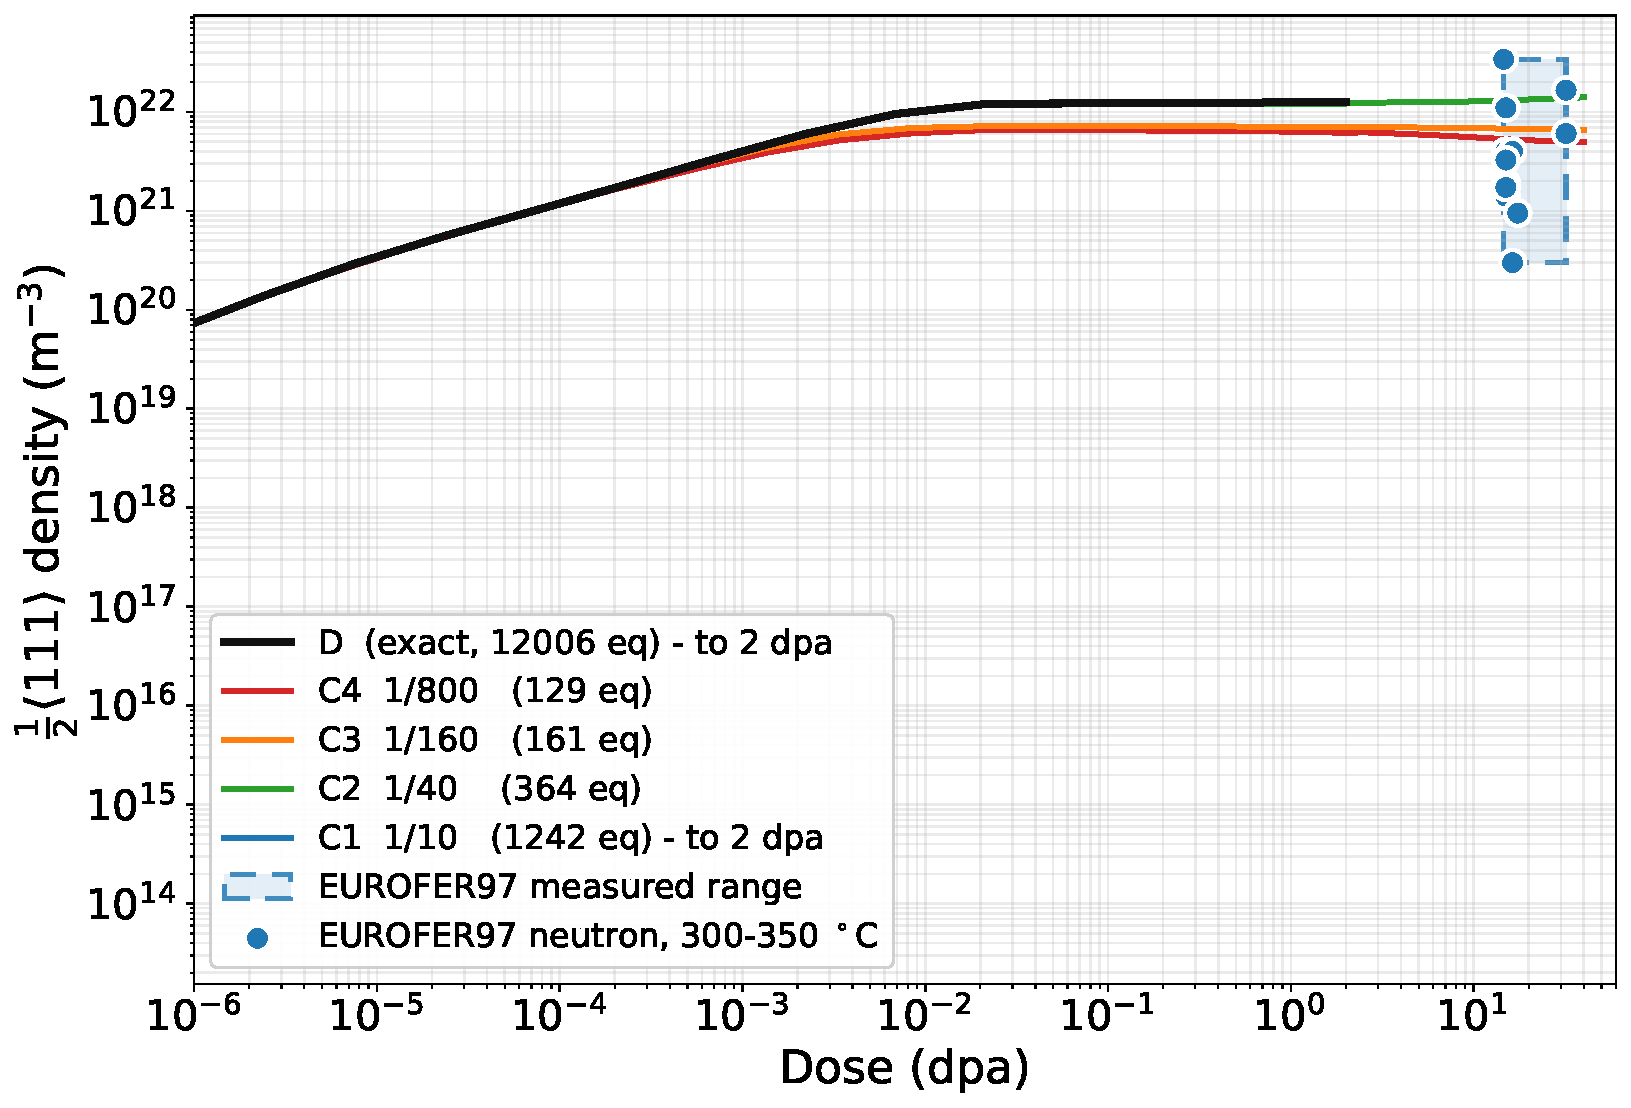
\includegraphics[width=0.86\textwidth]{figs/size_effect_N_loops_111.pdf}
\caption{\halfp{} loop number density. The exact solution separates from the
coarse rungs from \SI{0.1}{dpa} onward; C3 and C4 lose roughly half the
population.}\label{fig:n111}\end{figure}

\begin{figure}[htbp]\centering
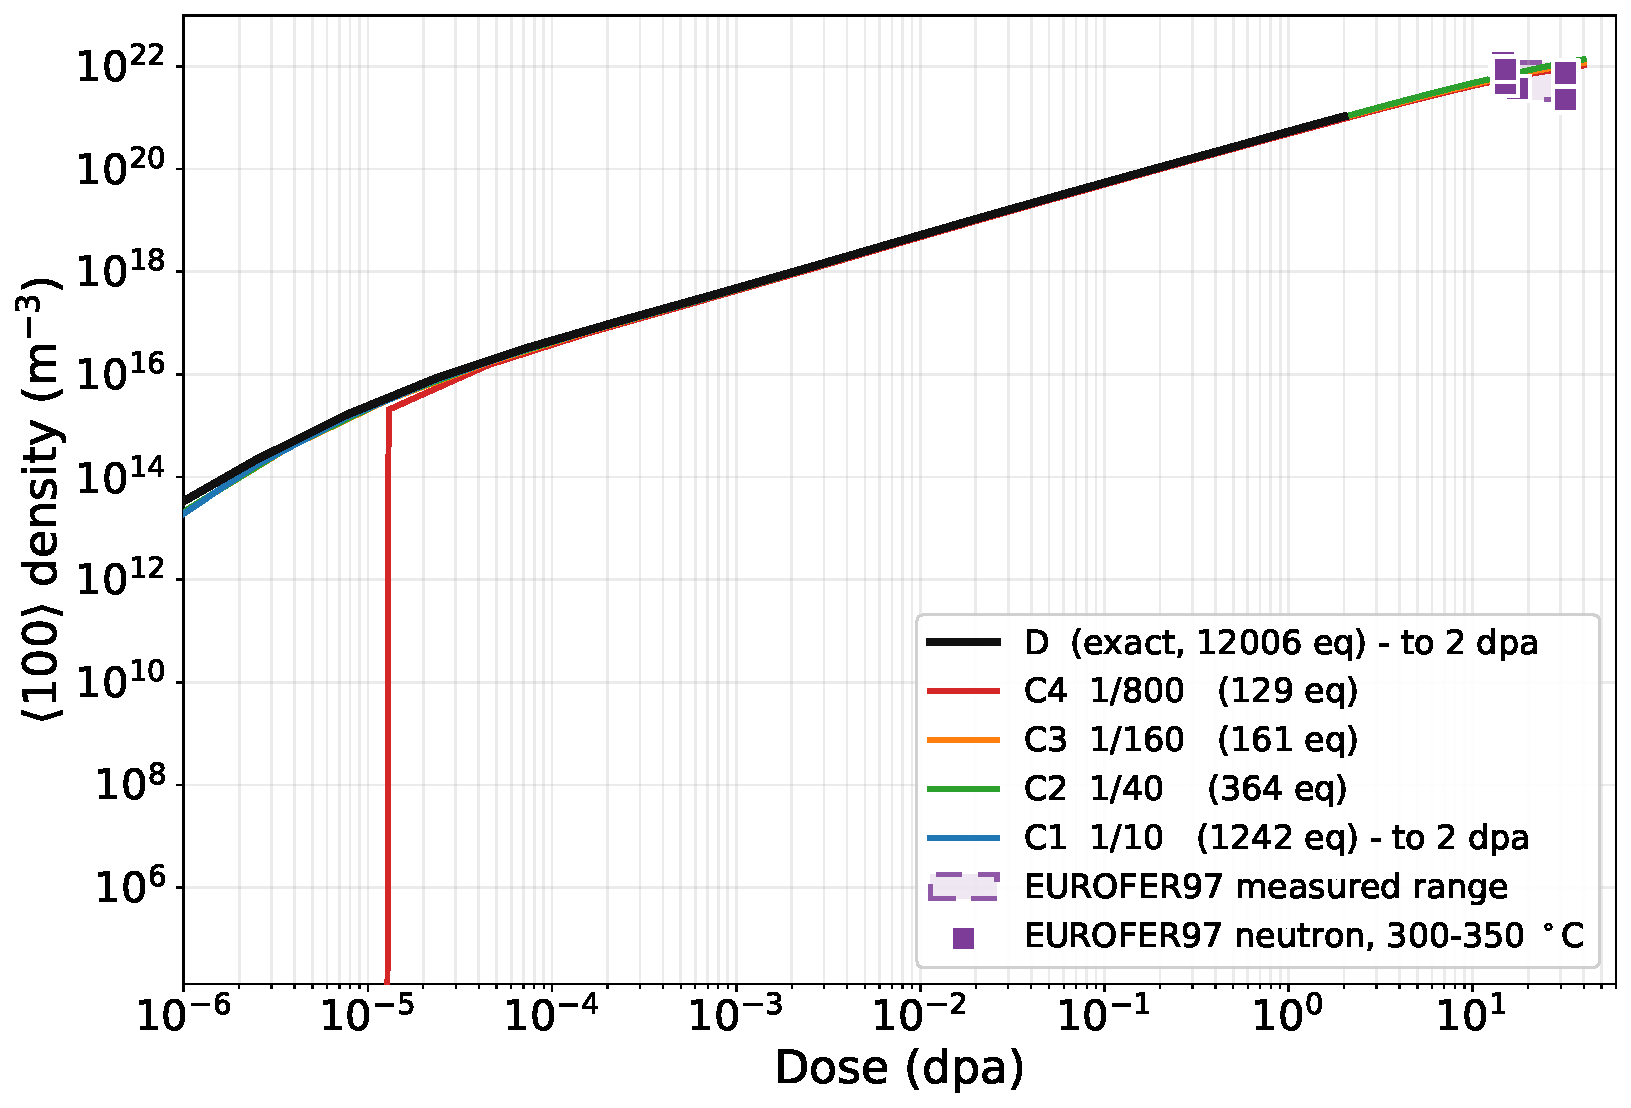
\includegraphics[width=0.86\textwidth]{figs/size_effect_N_loops_100.pdf}
\caption{\hkl{} loop number density. All rungs track the exact solution
closely; this is the observable the closure represents best.}\label{fig:n100}\end{figure}

\begin{figure}[htbp]\centering
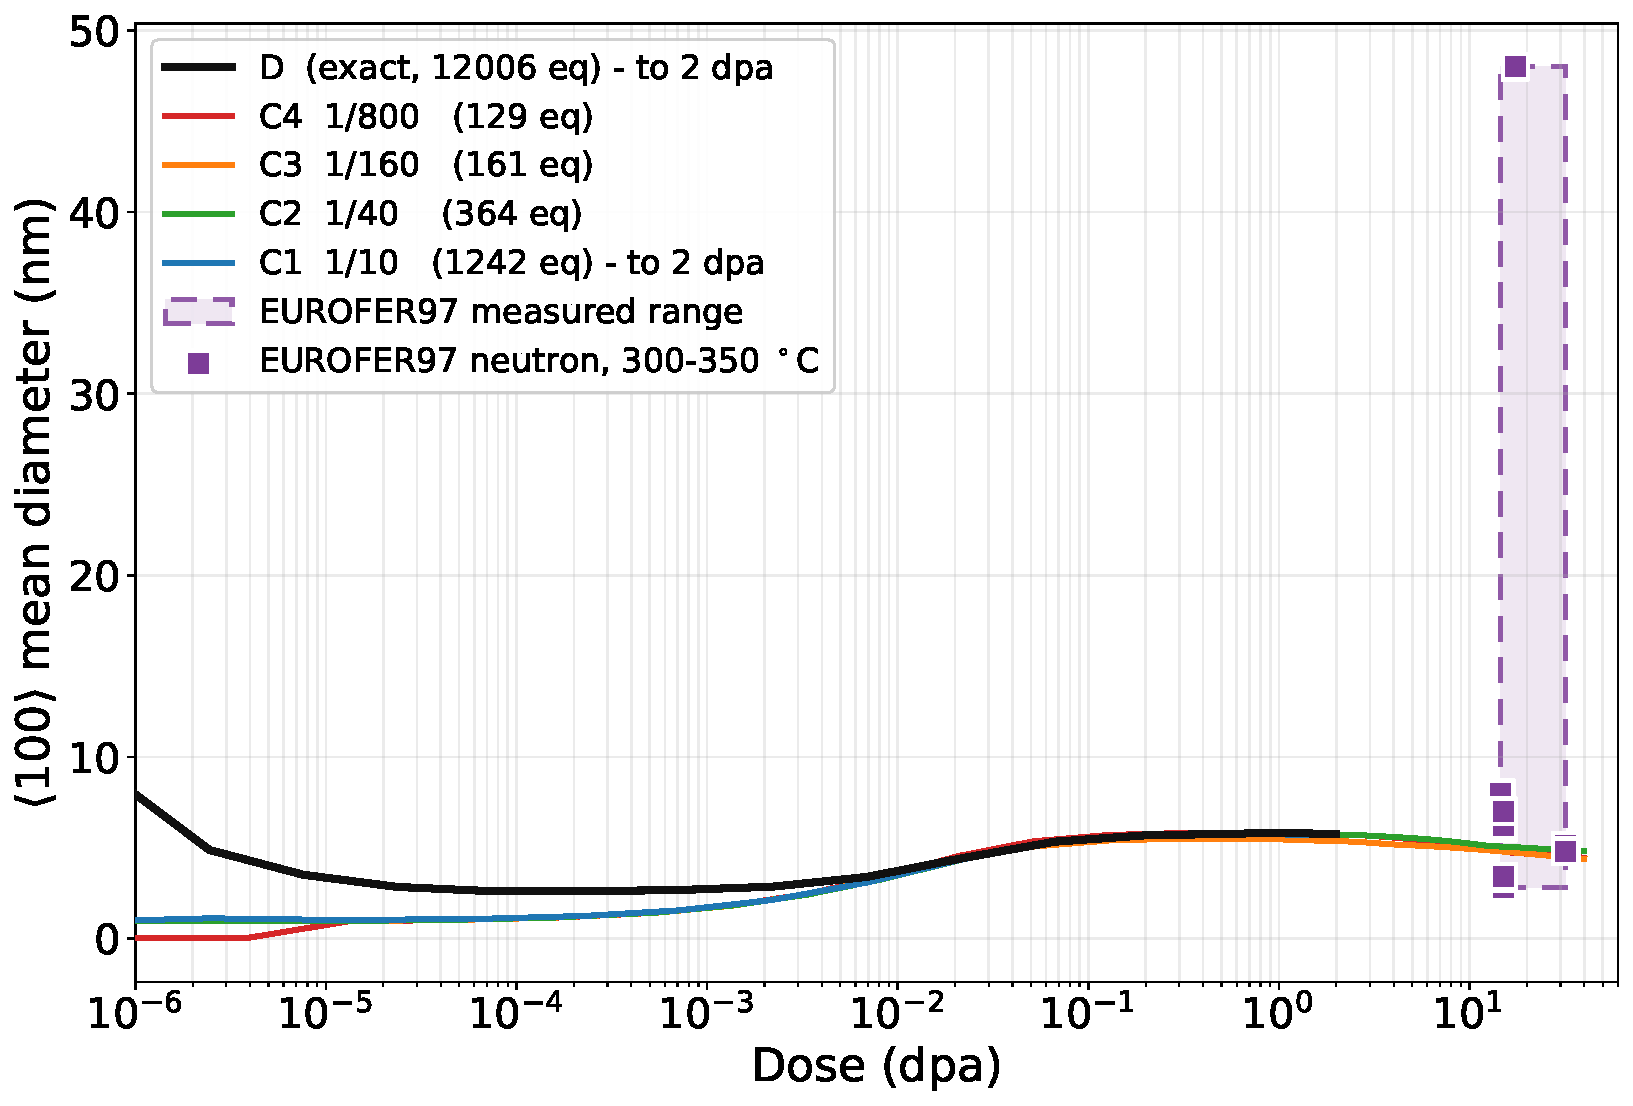
\includegraphics[width=0.86\textwidth]{figs/size_effect_d_100_nm.pdf}
\caption{\hkl{} mean diameter. Held to about one percent across the whole
ladder.}\label{fig:d100}\end{figure}

\begin{figure}[htbp]\centering
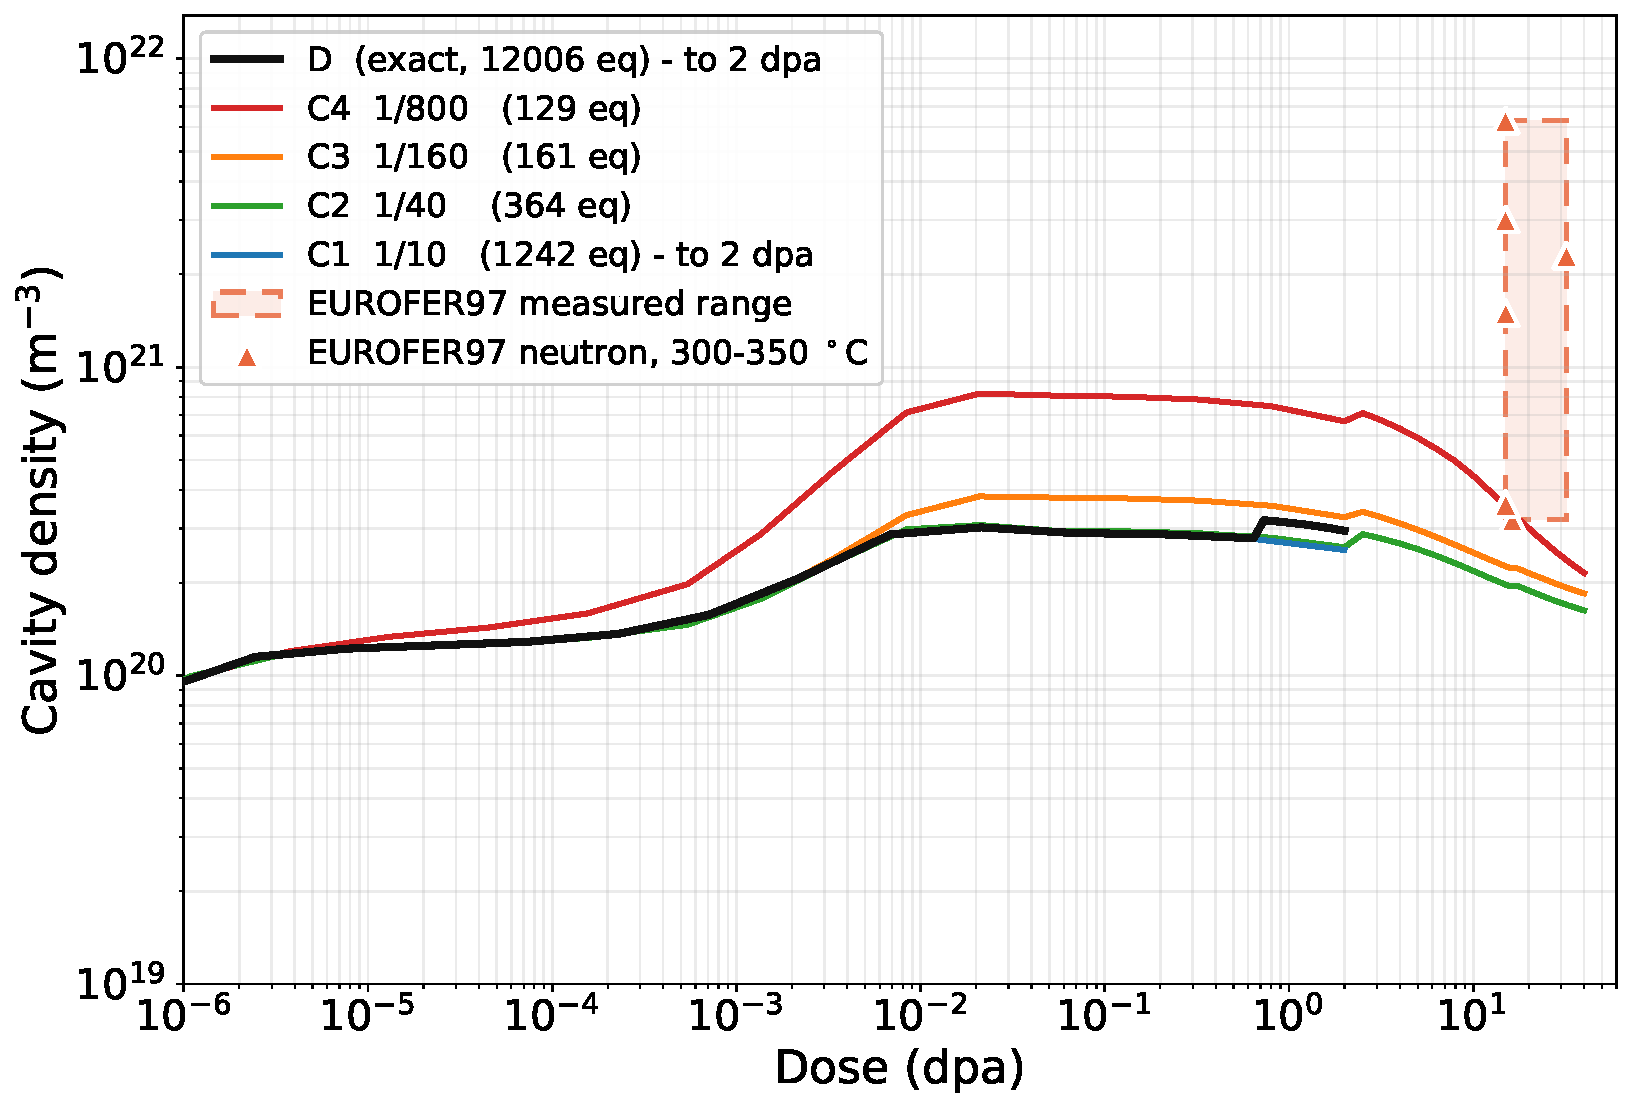
\includegraphics[width=0.86\textwidth]{figs/size_effect_N_voids.pdf}
\caption{Cavity number density --- the observable most sensitive to system
size, with C4 more than a factor of two above the exact
solution.}\label{fig:nvoids}\end{figure}

\begin{figure}[htbp]\centering
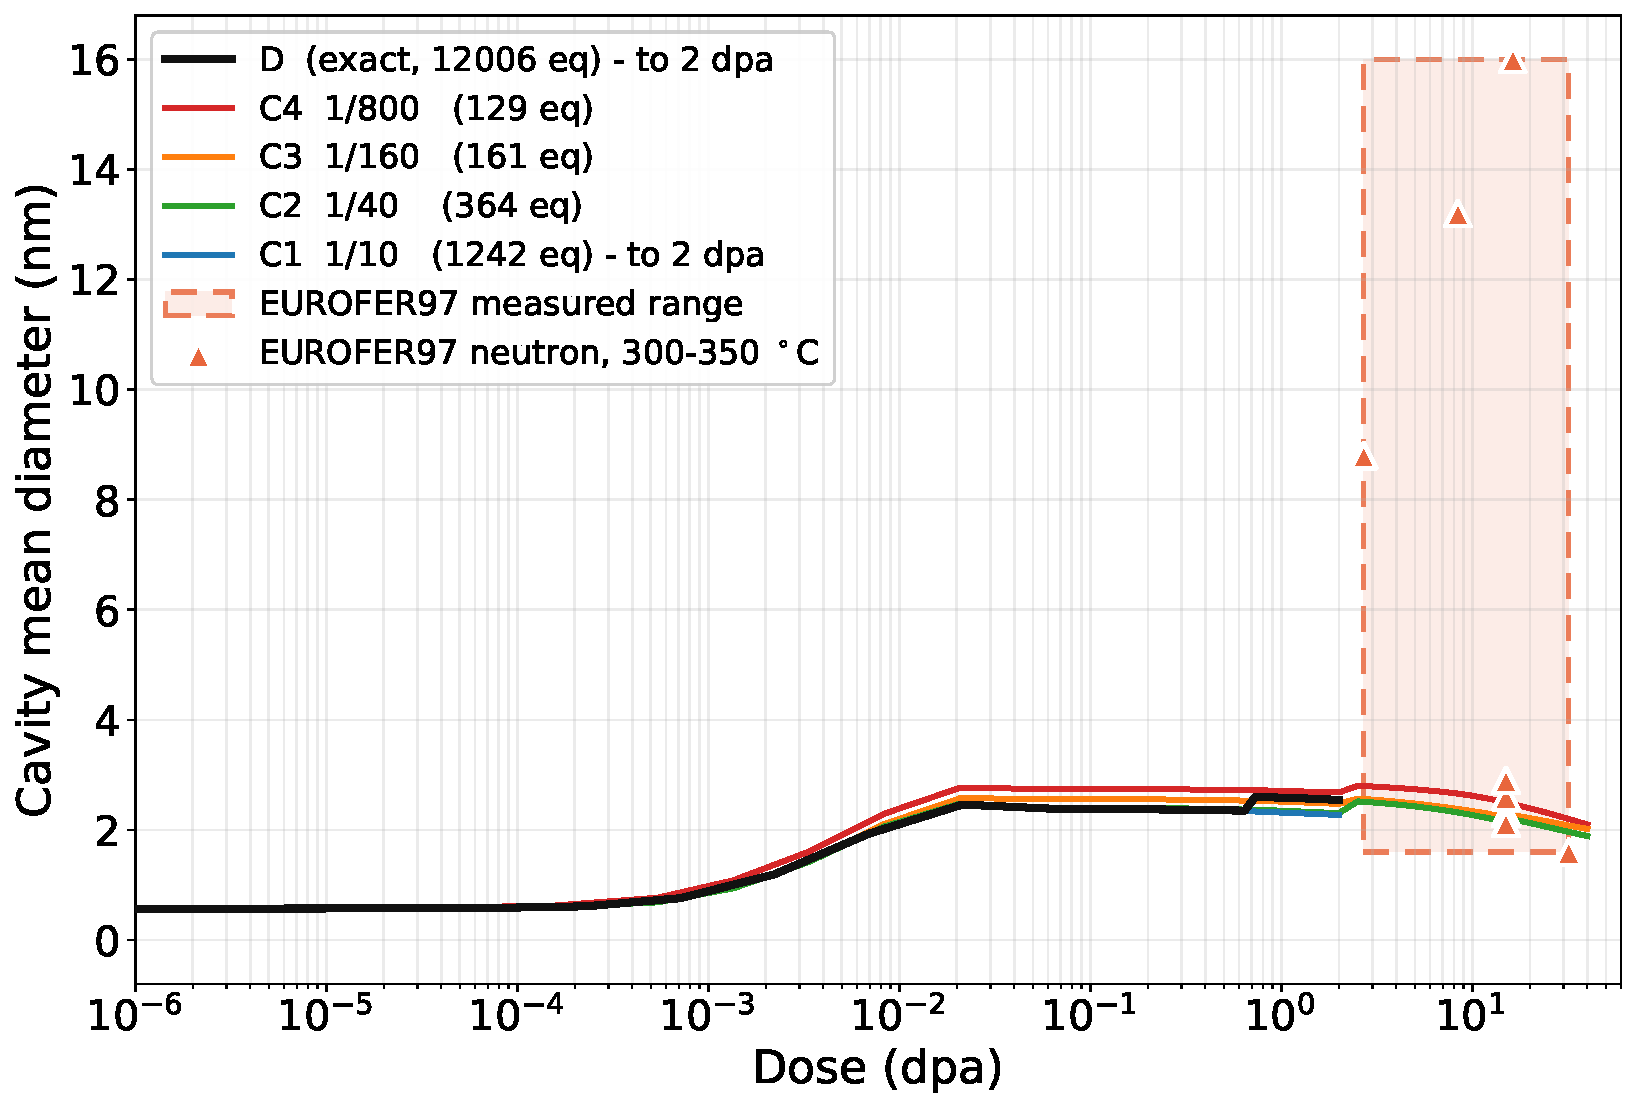
\includegraphics[width=0.86\textwidth]{figs/size_effect_d_cavity_nm.pdf}
\caption{Cavity mean diameter. The cavity data extend down to \SI{2.7}{dpa},
so this is the one panel where band and curves nearly
meet.}\label{fig:dcav}\end{figure}

\clearpage
%======================================================================
\section{Campaign M --- Separating System Size from Binning}\label{sec:campM}
%======================================================================

Table~4 measured closure error at one domain and one dose, because that was all
its exact arm could reach, and its rungs moved $i_{\rm discrete}$ and
$I_{\rm bin}$ \emph{together}. A deviation there cannot be attributed to either.
Campaign~M separates them: \textbf{M1} varies the domain with no closure at all,
\textbf{M2R} varies the bin count at fixed discrete core, and \textbf{M2D}
sweeps both independently so that every cell has a neighbour differing in
exactly one axis.

All of campaign~M runs at production mobility ($i_{\rm mobile} = v_{\rm mobile}
= 5$), fission cascade, \texttt{LOOP\_COAL} and \texttt{prec\_bw} at their
defaults in \emph{both} arms, on one shared 45-point logarithmic grid to
\SI{20}{dpa}.

\subsection{M1 --- what an exact arm costs}

\begin{table}[htbp]
\centering
\caption{Cost of the fully discrete arm against domain. The bold row is the
only one that completes, and it is the reference for everything below.}
\begin{tabular}{lrrrr}
\toprule
Run & $I=V$ & $N_{\rm eq}$ & Dose reached & Wall \\
\midrule
\bfseries M1\_D1000 & 1000 & 2006 & 20 / 20 & 5.2 min \\
M1\_D2000 & 2000 & 4006 & 0.03839 / 20 & 61.1 min \\
M1\_D4000 & 4000 & --- & \multicolumn{2}{c}{\itshape not run --- see text} \\
\bottomrule
\end{tabular}

\end{table}

The cliff is abrupt. Doubling the domain takes the exact arm from finishing in
five minutes to reaching \SI{0.2}{\percent} of the same dose in an hour, and at
$I=V=10\,000$ it diverges outright --- per-step cost growing $\approx4\times$
per output step, \SI{2643}{\second} on step 28 of 45, at
\SI{104}{\percent} CPU, i.e.\ entirely inside the serial region. That region is
\texttt{loop\_coal}'s $O(N_C^2)$ pair sum: the participation gate admits sessile
sizes above $2\,C_{\rm floor}$, and at $I=10\,000$ that population is
$\sim10\times$ the $I=1000$ one, so the pair count is $\sim100\times$. It is the
same failure that defeated the Table~4 exact arm three times.

Domains of 4000 and above were not attempted. Once 2000 misses by that margin
they cannot succeed, and each would cost an hour to confirm it.

\subsection{M2R --- bin count at the reference domain}

\begin{table}[htbp]
\centering
\caption{Deviation from the exact arm (\si{\percent}) at \SI{20}{dpa},
$I=V=1000$, $i_{\rm discrete} = v_{\rm discrete} = 50$ throughout. Only the bin
count varies.}
\begin{tabular}{lrrrrrrrr}
\toprule
Rung & $I_{\rm bin}$ & $r$ & $N_{\rm eq}$ & $N_{111}$ & $d_{111}$ & $N_{100}$ & $d_{100}$ & $d_{\rm cav}$ \\
\midrule
B2 & 2 & 4.47 & 114 & +3.7 & -4.4 & +1.2 & -0.6 & -2.7 \\
B3 & 3 & 2.71 & 118 & +1.8 & -5.4 & -2.1 & +1.0 & -2.1 \\
B4 & 4 & 2.11 & 122 & +1.4 & -5.3 & -1.2 & -5.4 & -2.4 \\
B6 & 6 & 1.65 & 130 & +1.2 & -5.8 & -2.1 & -2.3 & -1.6 \\
B8 & 8 & 1.45 & 138 & +1.1 & -6.3 & -1.2 & -0.8 & -0.8 \\
B12 & 13 & 1.28 & 158 & +1.0 & -4.8 & -0.2 & +0.1 & -0.1 \\
B16 & 17 & 1.21 & 174 & +0.9 & -5.4 & -0.1 & +0.3 & +0.1 \\
B24 & 25 & 1.13 & 206 & +1.0 & -6.4 & -0.2 & +0.1 & +0.1 \\
B32 & 33 & 1.10 & 238 & +1.0 & -6.6 & -0.2 & +0.1 & +0.1 \\
\bottomrule
\end{tabular}

\end{table}

Five of the six observables converge: by $I_{\rm bin} = 12$ ($N_{\rm eq} = 158$
against the exact 2006, a $13\times$ reduction) $N_{100}$, $d_{100}$,
$N_{\rm cav}$ and $d_{\rm cav}$ are all inside \SI{0.3}{\percent}, and $N_{111}$
plateaus at a residual $+\SI{1.0}{\percent}$.

$d_{111}$ does not. It sits at $-5$ to $-\SI{6.6}{\percent}$ and does
\emph{not} improve --- the finest rung is the worst of the nine. Section
\ref{sec:d111} explains why, and it is not a defect in the closure.

\subsection{M2D --- the two-dimensional sweep}\label{sec:m2d}

\begin{table}[htbp]
\centering
\caption{$d_{111}$ deviation from the exact arm (\si{\percent}) at
\SI{20}{dpa}. Read \emph{down} a column, not across a row: the error falls with
$i_{\rm discrete}$ and is nearly flat in $I_{\rm bin}$.}
\begin{tabular}{lrrrr}
\toprule
$i_{\rm discrete}$ & $I_{\rm bin}=4$ & $I_{\rm bin}=8$ & $I_{\rm bin}=16$ & $I_{\rm bin}=32$ \\
\midrule
25 & -7.2 & \dnr & -6.7 & \dnr \\
50 & -5.3 & -6.3 & -5.4 & \dnr \\
100 & \dnr & \dnr & \dnr & \dnr \\
200 & \dnr & \dnr & \dnr & \dnr \\
400 & \dnr & \dnr & \dnr & \dnr \\
800 & \dnr & \dnr & \dnr & \dnr \\
\bottomrule
\end{tabular}

\end{table}

\begin{table}[htbp]
\centering
\caption{$d_{\rm cav}$ deviation (\si{\percent}) over the same sweep, for
contrast --- converged almost everywhere, with one anomaly discussed below.}
\begin{tabular}{lrrrr}
\toprule
$i_{\rm discrete}$ & $I_{\rm bin}=4$ & $I_{\rm bin}=8$ & $I_{\rm bin}=16$ & $I_{\rm bin}=32$ \\
\midrule
25 & -2.7 & \dnr & +0.1 & +0.0 \\
50 & -2.4 & -0.8 & +0.1 & +0.1 \\
100 & \dnr & -0.3 & -0.0 & +0.0 \\
200 & +15.1 & -0.2 & -0.1 & -0.1 \\
400 & \dnr & -0.2 & \dnr & -0.1 \\
800 & -0.1 & -0.1 & -0.0 & \nreal \\
\bottomrule
\end{tabular}

\end{table}

\noindent
\textbf{Reading the grid.} \dnr{} marks a cell that hit the one-hour cap short
of \SI{20}{dpa} and is therefore refused as a metric (\S3.4.1); it is a cost
result, not a method failure. \nreal{} marks a configuration the bin layout
cannot realise: at $i_{\rm discrete} = 800$ only 200 sizes remain for the bins,
so $I_{\rm bin} = 32$ returns 24 and the layout check \emph{raises} rather than
running a different grid than the one requested. That guard exists because nine
bit-identical ``refinement'' runs were once produced by a silently dropped bin
configuration.

Read \emph{down} column $I_{\rm bin} = 8$: $-6.3$, $-3.4$, $-2.0$, $-0.1$,
$+0.7$. Read \emph{across} row $i_{\rm discrete} = 100$: $-3.4$, $-4.2$,
$-5.1$ --- worse with every bin added. The bottom row, $i_{\rm discrete} = 800$,
is converged to under \SI{1}{\percent} on $d_{111}$ at \emph{every} bin count.
The axis that matters is not the one the M2R ladder swept.

\subsection*{One anomalous cell}

$i_{\rm discrete} = 200$, $I_{\rm bin} = 4$ gives $d_{\rm cav}$
$+\SI{15.1}{\percent}$ where its row-neighbours sit at $-\SI{0.2}{\percent}$,
with $N_{\rm cav}$ and $\overline{n}_v$ both $+\SI{52}{\percent}$. It ran in
\SI{6}{\second} against \SIrange{39}{46}{\minute} for those neighbours, and it
reproduces exactly on a standalone re-run. Coarse bins make the system
non-stiff, which explains the speed; they do not explain the error, because the
\emph{coarser} $I_{\rm bin} = 4$ cells at $i_{\rm discrete} = 25$ and 50 give
$-2.7$ and $-\SI{2.4}{\percent}$. The cause is \textbf{not established}. It is
recorded here rather than smoothed over, and it is the same non-monotonicity
Table~4 showed when C3 came out worse than C2 --- with a sharper example.

\subsection{Why $d_{111}$ does not converge in bin count}\label{sec:d111}

\textbf{The M2R ladder turned the knob that does not control this error.} The
\halfp{} mean-size error converges in $i_{\rm discrete}$, not in $I_{\rm bin}$,
and $i_{\rm discrete} = 50$ was held fixed across all nine rungs.

At fixed $I_{\rm bin} = 16$ and \SI{0.05}{dpa}, against an exact
$d_{111} = \SI{2.9787}{\nano\metre}$, the error tracks the fraction of the
\halfp{} \emph{content} that lies above the discrete core --- i.e.\ the fraction
the closure has to represent:

\begin{center}
\begin{tabular}{rrr}
\toprule
$i_{\rm discrete}$ & $d_{111}$ (\si{\nano\metre}) & \% of content binned \\
\midrule
25  & 2.7232 \quad($-8.6\%$) & 96.6 \\
50  & 2.7744 \quad($-6.9\%$) & 91.2 \\
100 & 2.8128 \quad($-5.6\%$) & 83.4 \\
200 & 2.8692 \quad($-3.7\%$) & 70.6 \\
400 & 2.9403 \quad($-1.3\%$) & 47.7 \\
800 & 2.9813 \quad($+0.1\%$) & \phantom{0}8.0 \\
\bottomrule
\end{tabular}
\end{center}

This is ordinary closure error; it simply converges along the axis that was held
fixed. Conversely, at fixed $i_{\rm discrete} = 400$, raising $I_{\rm bin}$ from
4 to 8 to 33 gives 2.9615, 2.9503, 2.9245 --- \emph{slightly worse}.

Nothing is special about \halfp{}. Its mean size is $\approx147$ SIAs, about
$3\times$ the discrete core, so the peak of the distribution sits inside the
binned region and the closure carries it. $d_{100}$ and $d_{\rm cav}$ improve
monotonically along the same sweep with about a tenth the amplitude.

Four explanations were tested and rejected, each by measurement:

\begin{itemize}
\item \textbf{Not a code-path difference.} With $I_{\rm bin} = 0$ and
$i_{\rm discrete} = I$ --- the bin-moment path carrying no closure --- it
reproduces the discrete arm at \SI{20}{dpa} to within rounding on all six
observables ($d_{111}$ $-0.000\%$, $\delta_{\rm FP}$ $+0.001\%$).
\texttt{check\_bm\_vs\_discrete.py} asks this at \SI{1e-2}{dpa}; this extends it
three decades, to the dose where the deviation is measured.
\item \textbf{Not \texttt{LOOP\_COAL}.} It was the leading suspect, being the
only channel implemented twice and the only one that moves content up in size
space by large jumps. With it \emph{off in both arms} the deficit is unchanged:
$-7.3\%$ and $-7.0\%$, against $-7.0\%$ and $-7.9\%$ with it on.
\item \textbf{Not a domain-edge artefact.} The exact spectrum decays smoothly to
the top of the grid --- size 1000 holds \SI{0.01}{\percent} of the content, with
no pile-up --- so the edge-piling convention is not implicated.
\item \textbf{Not slow accumulation.} The deficit is already $-8.4\%$ at
\SI{0.005}{dpa}, the first meaningful output point, and drifts only to $-6.6\%$
by \SI{20}{dpa}.
\end{itemize}

\begin{figure}[htbp]
\centering
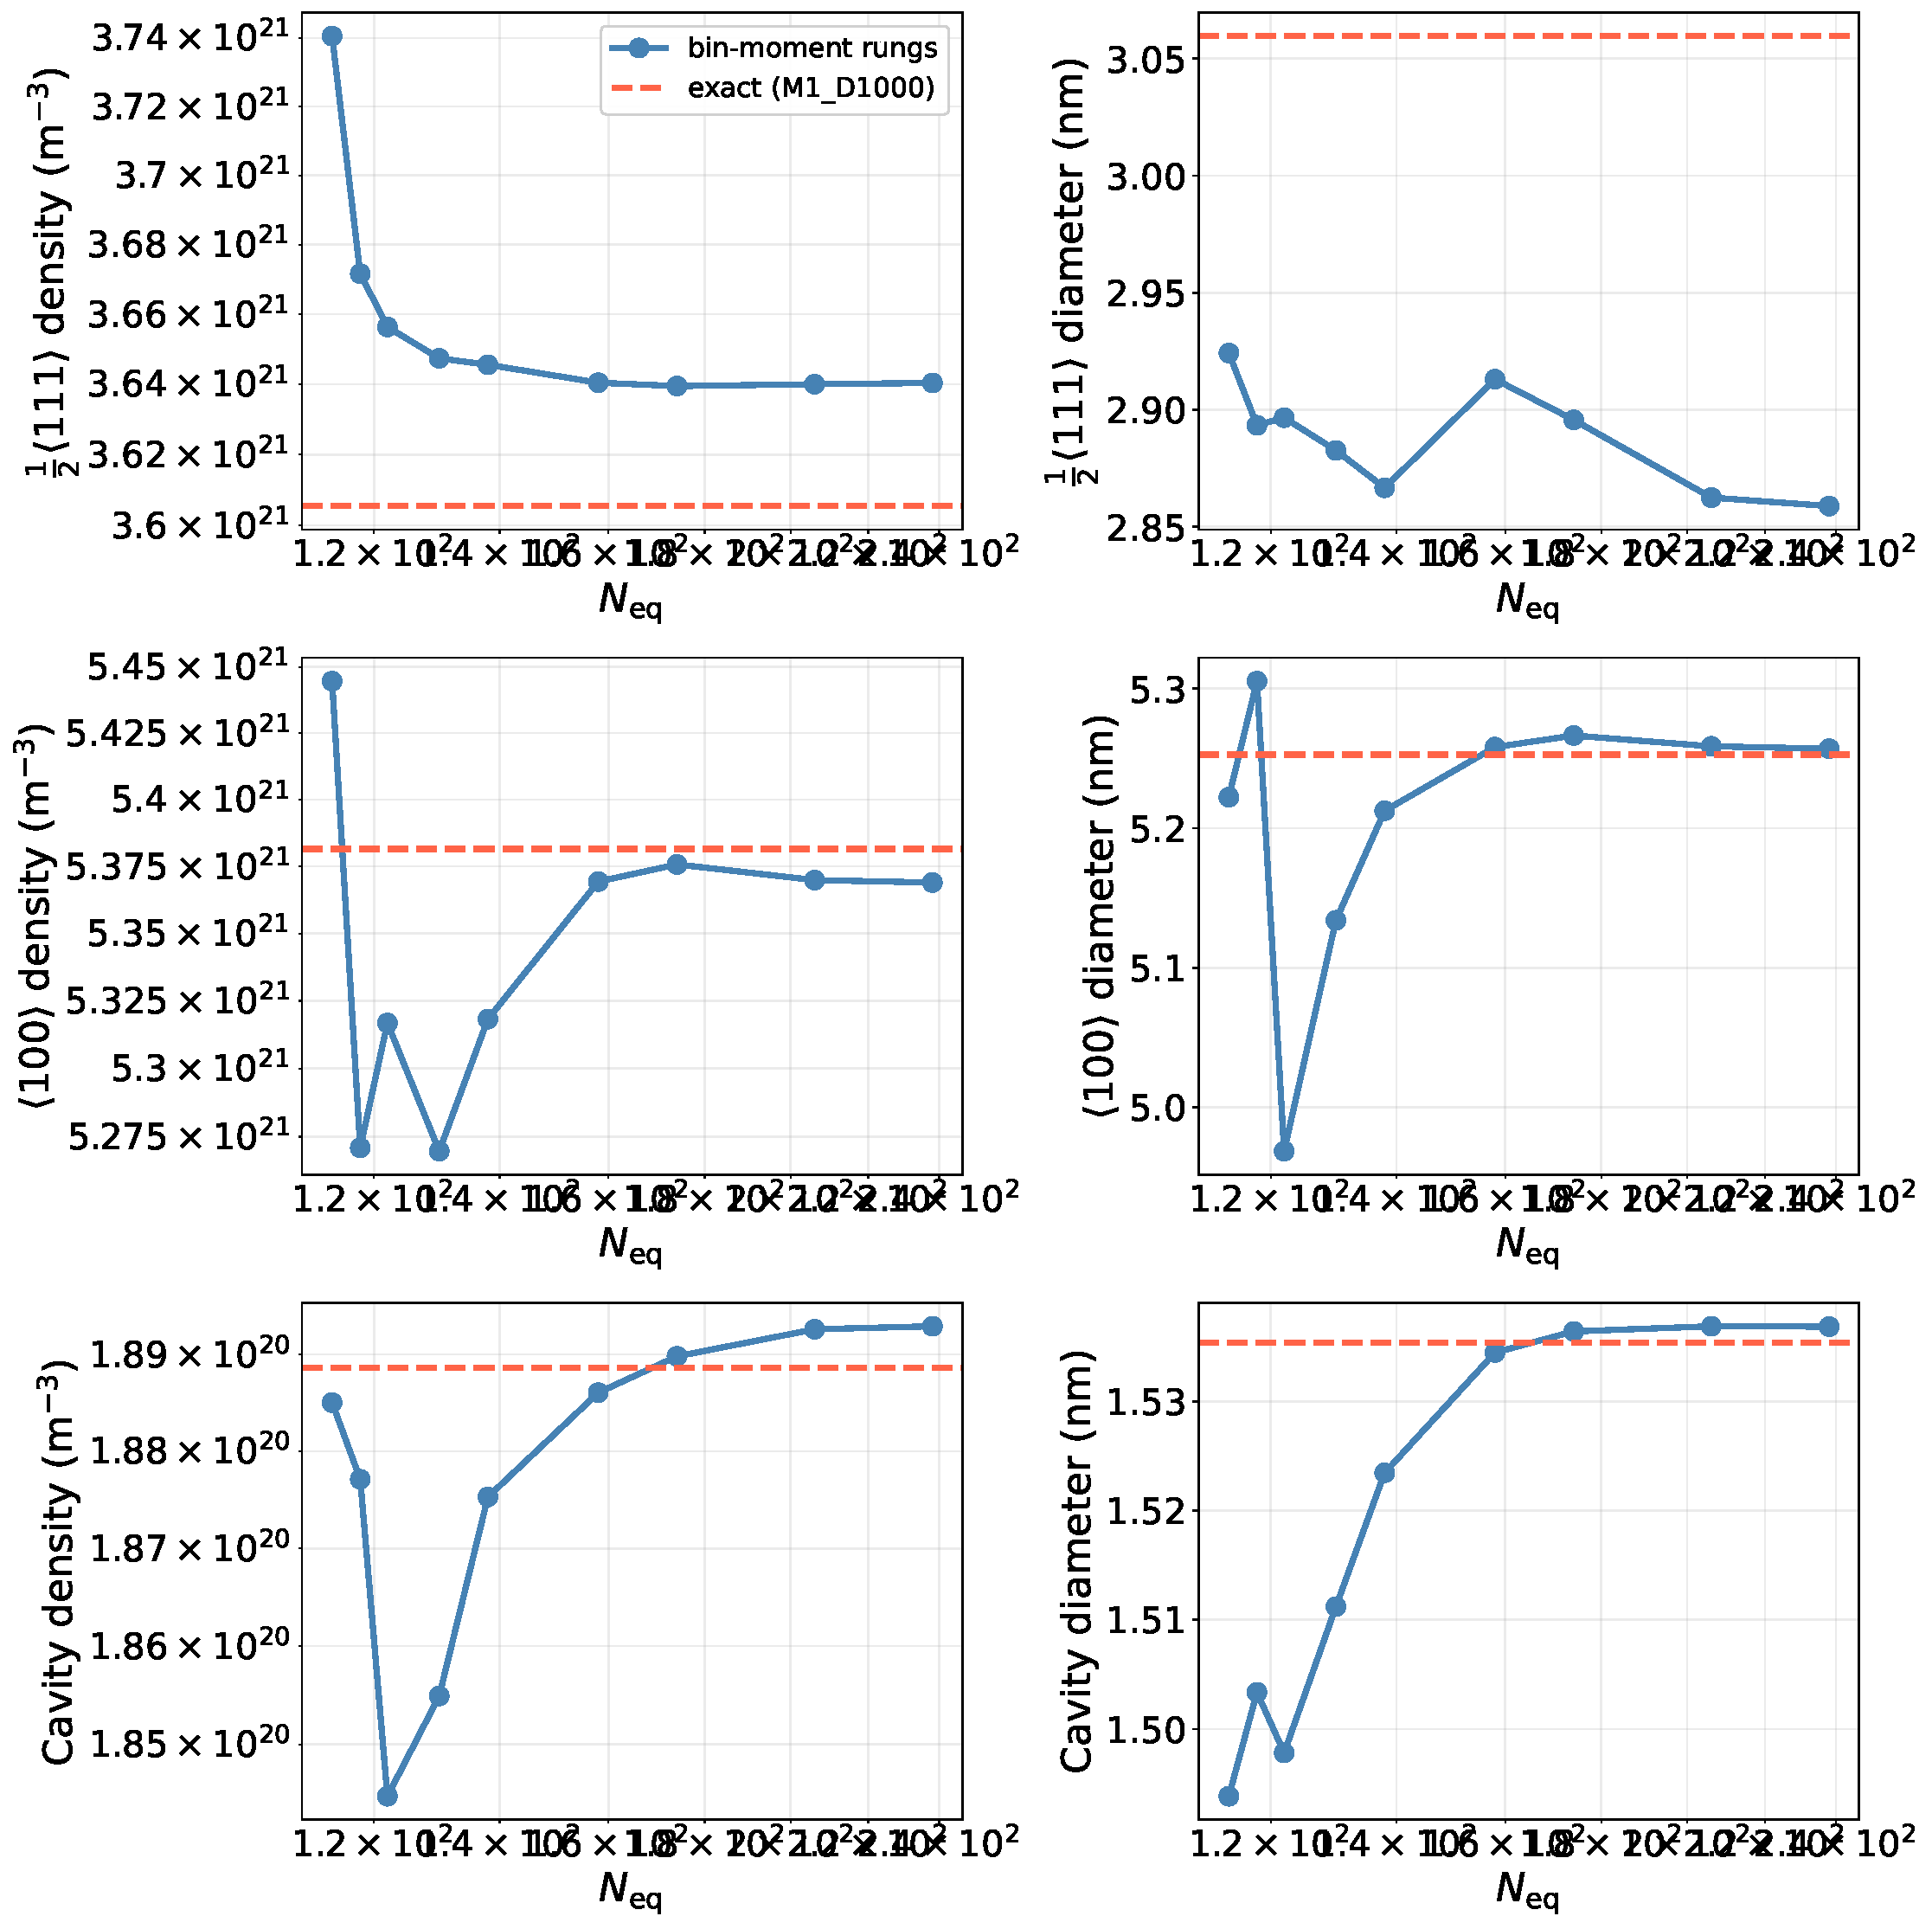
\includegraphics[width=0.98\textwidth]{figs/M_convergence.pdf}
\caption{M2R: the six observables against $N_{\rm eq}$ at fixed
$i_{\rm discrete} = 50$, with the exact arm as the dashed line. Five panels
close on it; $d_{111}$ runs parallel to it and never approaches.}
\end{figure}

\begin{figure}[htbp]
\centering
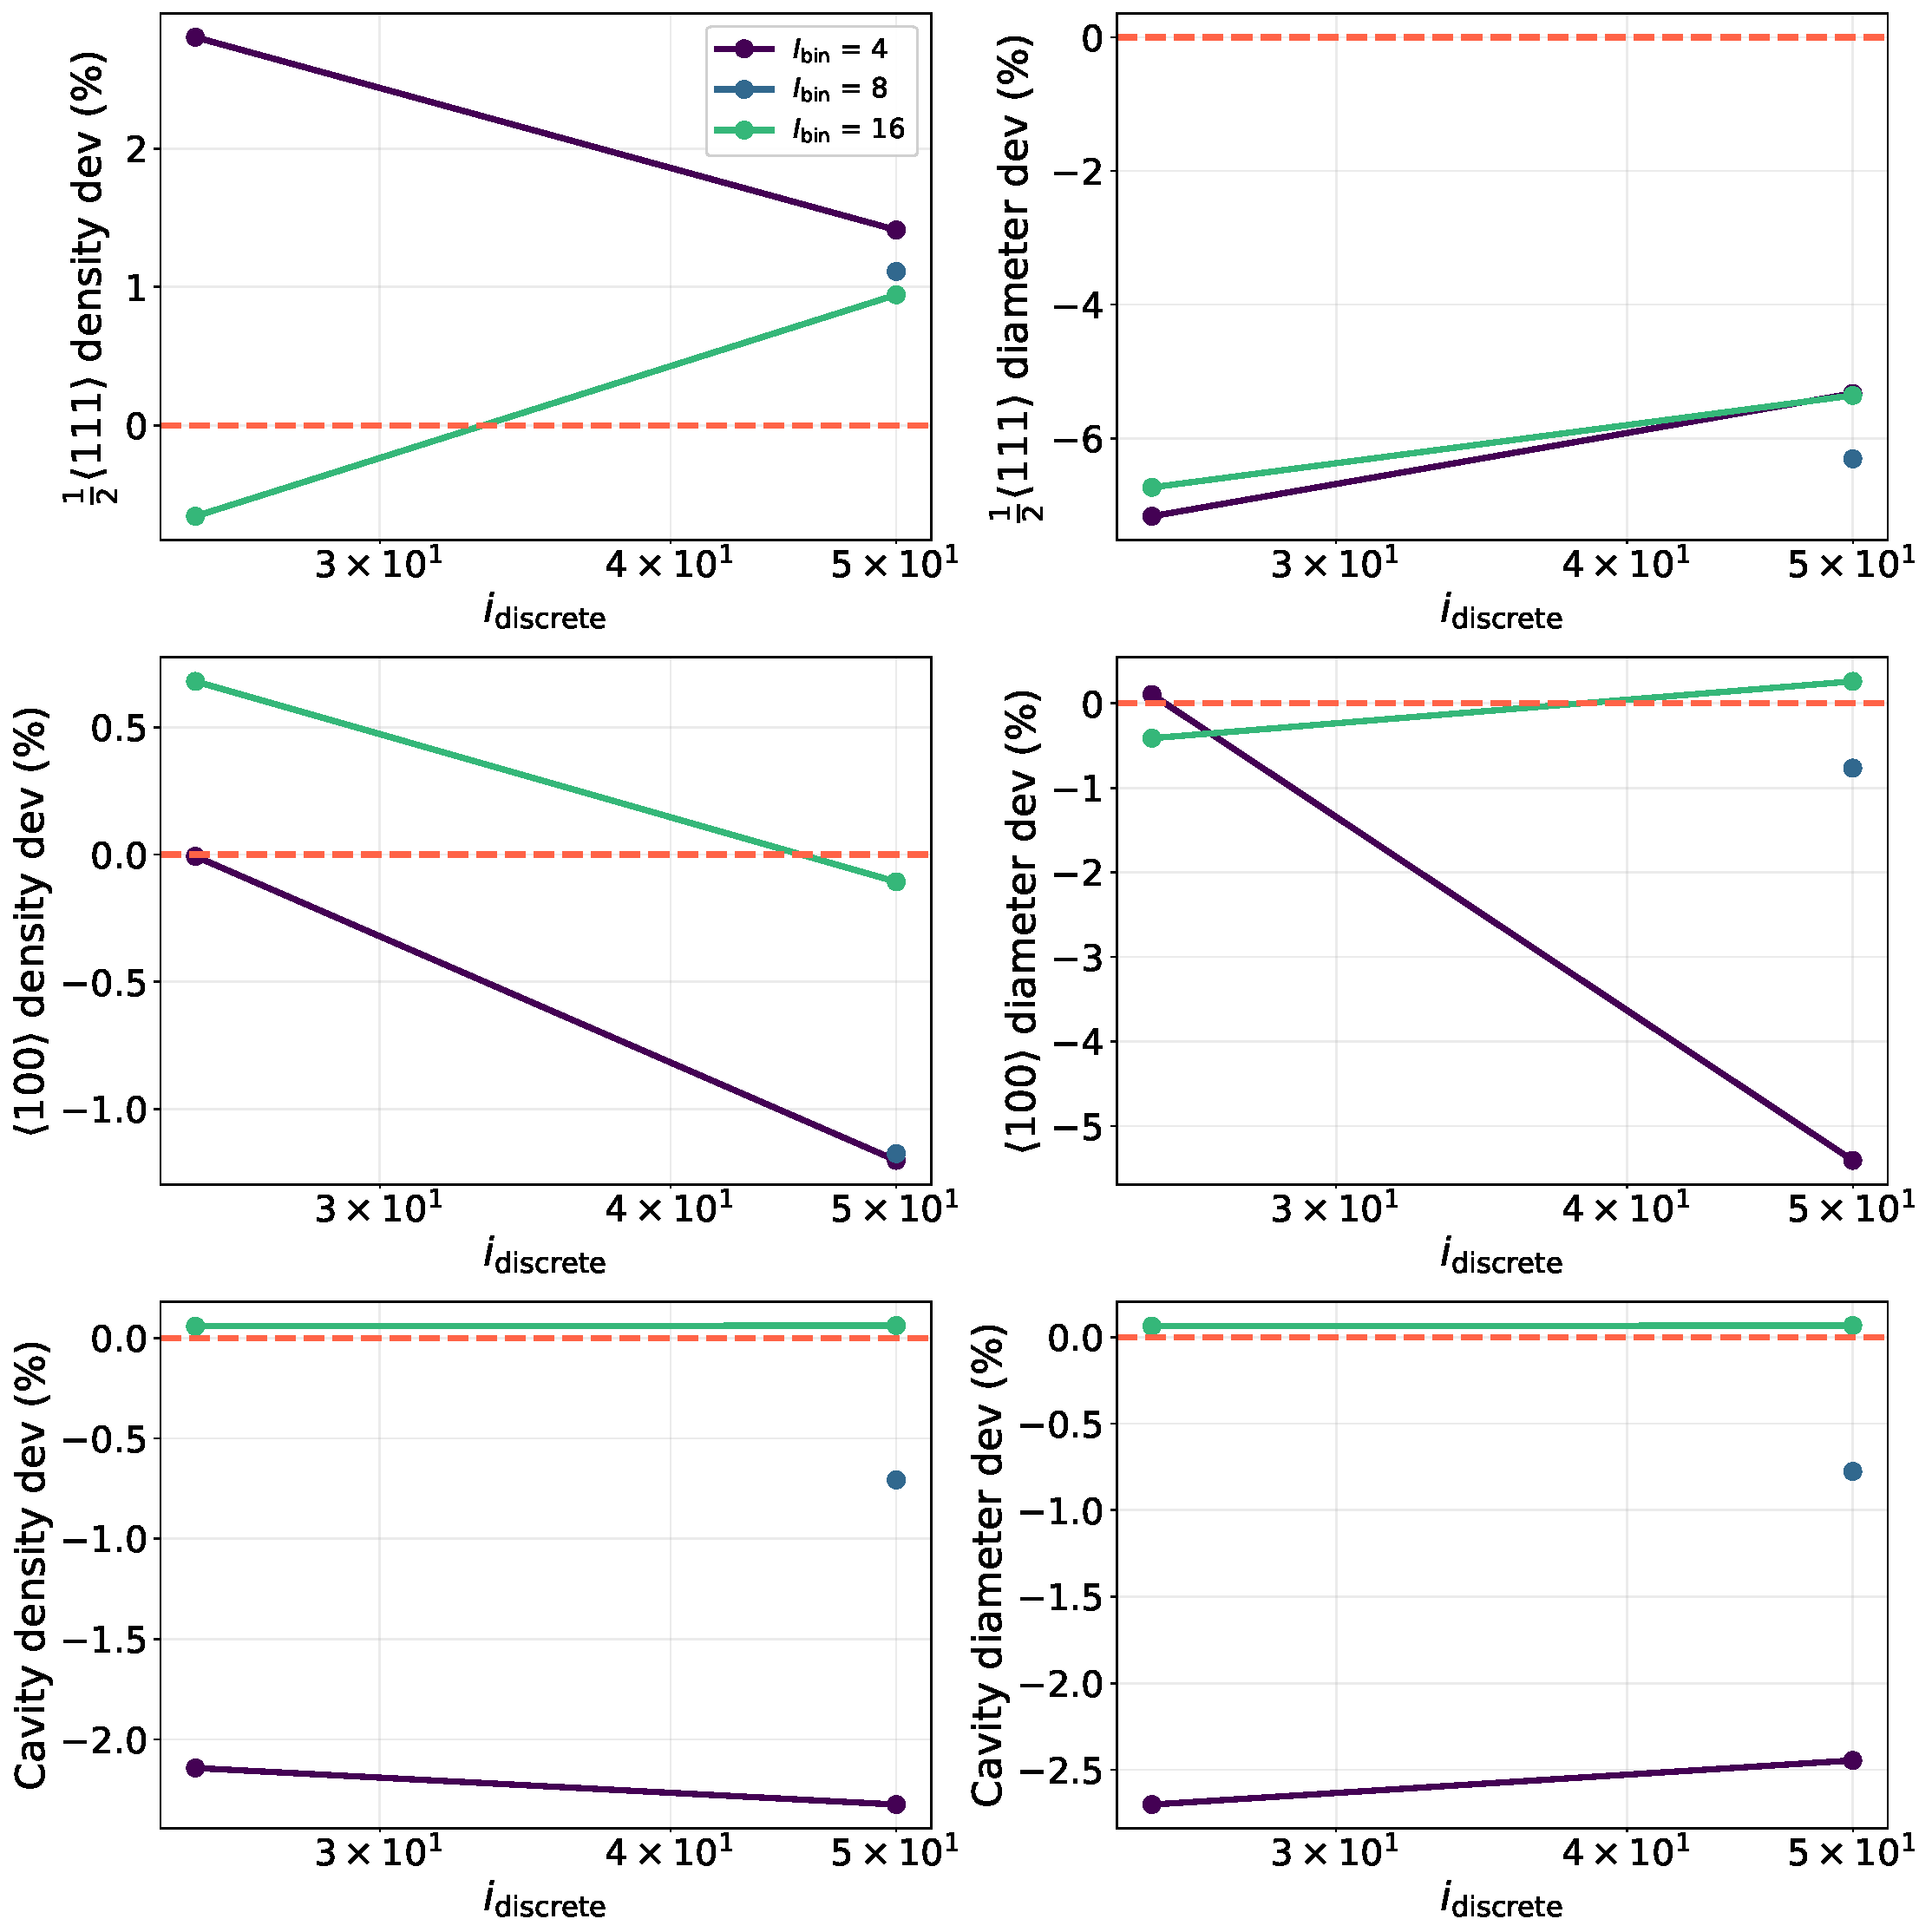
\includegraphics[width=0.98\textwidth]{figs/M_2d_sweep.pdf}
\caption{M2D: deviation against $i_{\rm discrete}$, one curve per
$I_{\rm bin}$. The curves collapse onto one another --- the spread
\emph{between} bin counts at fixed $i_{\rm discrete}$ is small next to the fall
\emph{along} $i_{\rm discrete}$. This is the figure the M2R ladder could not
draw, because it moved along a contour of this surface rather than down it.}
\end{figure}

\subsection{What this means for choosing a grid}

\begin{enumerate}
\item \textbf{A binning study must sweep both axes.} Table~4 moved them
together and confounded them; M2R moved one and hid an error in the other.
Neither design can attribute a deviation.
\item \textbf{$i_{\rm discrete}$ should be chosen against the population's mean
size}, not set to a fixed number. $i_{\rm discrete} = 50$ with a mean of 147
puts the peak of the distribution inside the closure.
\item \textbf{Cost is not monotonic in either axis.} At \SI{0.05}{dpa} the pure
discrete solve ran in \SI{13.8}{\second} and $i_{\rm discrete} = 50$,
$I_{\rm bin} = 16$ in \SI{4.2}{\second}, but $i_{\rm discrete} = 400$,
$I_{\rm bin} = 16$ took \SI{163.7}{\second} --- an order of magnitude slower
than either pure form, because the bin-moment path carries an
$O(i_{\rm discrete}^2)$ discrete--discrete coalescence block \emph{on top of}
the binned machinery. The accurate hybrid is the expensive one.
\end{enumerate}

\clearpage
%======================================================================
\section{Limitations}\label{sec:limits}
%======================================================================

\begin{enumerate}

\item \textbf{Table 4 verifies a variant of the model, not the production
configuration.} Production runs with \texttt{LOOP\_COAL~=~1}, the \halfp{}
loop--loop coarsening channel. That channel was implemented only in the
bin-moment solver path; the discrete path accepted the flag, recorded it in
provenance, and ignored it. The discrete arm was therefore never the exact
solution of the same equations, and the first version of this table
--- which showed a 90--114\% ``closure error'' on $d_{111}$ --- was measuring
the missing channel. The channel has since been implemented in the discrete
path and the two paths verified to agree to $7\times10^{-8}$
(\texttt{codes/Python\_Testing/check\_bm\_vs\_discrete.py}), but the
production-configuration exact arm proved unaffordable: the coarsening term is
$O(N_C^2)$ in the number of populated sessile sizes and, even gated, spent
\SI{2.8}{\hour} on a single output step at \SI{0.014}{dpa} of 2. Table~4 is
therefore run with the channel disabled in \emph{both} arms. The closure error
it measures is not demonstrably the production run's closure error.

\item \textbf{The no-coarsening variant is unphysical.} Without the channel the
\halfp{} mean size pins at the mobility cutoff and the loop density runs
20--60$\times$ over the EUROFER97 data. This does not invalidate the
verification --- verification asks whether the closure reproduces the exact
solution of the \emph{same} equations, which these two arms do --- but nothing
in Table~4 may be compared with experiment.

\item \textbf{Four columns never reached their comparison dose}: Table~1's B1,
Table~2's $P=3$ and $I_{\rm bin}$ 40, and Table~3's fusion+dynamic. Each is
reported with the dose it achieved. The reporting tool refuses to print a
metric for such a run, so this rule is mechanical rather than a matter of
discipline.

\item \textbf{$\delta_{\rm FP} \approx 0.05$--$0.07$ throughout}, against the
model's own $10^{-2}$ gate, and 0.158 for the two $P=1$/fusion columns. This is
a separate, disclosed defect. A verification study measures closure error
against the same equations; conservation error is not that, and the two should
not be conflated.

\item \textbf{$C_{\rm SIA,tot}$ is inflated 17--25$\times$ in fine-bin runs}
($I_{\rm bin} \ge 16$). When the top bin empties, its $\mu_0$ falls to the
$C_{\rm floor}$ level while its $\mu_1$ does not, leaving $\mu_1/\mu_0 \sim
10^8$ in a bin spanning 946--1001 --- a mean size arithmetically impossible for
that bin. \texttt{post\_process} already guards the \emph{mean-size} path
(\texttt{\_floor\_bin\_moments} clamps $\mu_1/\mu_0$ back inside the bin, a
guard added after \texttt{mean\_n\_100} once read 2853 on a grid of 1000), but
\texttt{SIA\_content\_from\_mu1} sums the \emph{raw} $\mu_1$, so the
corruption reaches $C_{\rm SIA,tot}$ unguarded. The six observables,
$\delta_{\rm FP}$ and swelling are unaffected; what breaks is the swelling
identity $S = S_I + \Delta J^d$, since $C_{\rm SIA,tot}$ is $S_I$. Reported,
not fixed.

\item \textbf{Campaign M's reference is a small domain.} $V = 1000$ caps a
cavity at about \SI{2.8}{\nano\metre} and the exact arm reports
$d_{\rm cav} = \SI{1.74}{\nano\metre}$ at \SI{20}{dpa} --- 62\% of the
ceiling. Both arms sit on the same truncated domain, so this cancels out of the
closure error being measured, but nothing in Section~\ref{sec:campM} may be
compared with experiment.

\item \textbf{An earlier dose-ladder defect invalidated a first round of
results.} The output grid held no point at the scoring dose, so a requested
\SI{15.72}{dpa} was silently scored at \SI{11.51}{dpa} (26.8\% low) while the
run reported having reached it. All affected rows were recomputed. This is the
same failure mode as the Figure~8 defect the study was commissioned to answer,
found inside the study's own tooling.

\end{enumerate}

\end{document}
